\section{Experimental Results and Analysis}
\subsection{SARS-CoV-1 Dataset}
The first dataset we use for CVAE-Casper Algorithm is SARS-CoV dataset from B. Sumudu U. Mendis1, Tamás D. Gedeon1, László T. Kóczy ~\cite{dataset1_2005}, which is a tiny dataset containing physiological indicator data. One datapoint here is a 23-dimension data, and the range of each element has already been normalized. For example, temperature at 8am has three attributes: slight, medium, high, and they are normalized by default. Also, there isn’t any noise datapoints in the dataset. In SARS-CoV dataset, there are 4000 datapoints for 4 labels: SARS patients, Normal people, High BP patients and Pneumonia patients. Since some of the attributes are so iconic that if some conditions are satisfied, we can directly assert the label of the datapoint, e.g. Only SARS patients have abdominal pain, high body temperature and nausea at the same time. Therefore, this classifier problem will become a linear problem and no need to use neural networks. Also, some physiologic indexes like blood pressure are hard for people to track in daily life. Hence, we try to choose only body temperature by time as the input data. Also, body temperature is significant medical data which are easy to track and highly related to SARS. ~\cite{covidfeatures2020} As a result, the dimension of the input data will be 12 which are sequential body temperatures. A quick peek of the data is as follows.


\begin{table}
\begin{tabular}{|l|l|l|l|l|l|l|l|l|l|l|l|}
\hline
\multicolumn{3}{|l|}{Temp 8am} & \multicolumn{3}{l|}{Temp 12pm} & \multicolumn{3}{l|}{Temp 4pm} & \multicolumn{3}{l|}{Temp 8pm} \\ \hline
       slight&      medium&         high&   slight&      medium&      high&  slight&      medium&      high& slight&   medium& high             \\ \hline
       0.1013&       0.929&       0.842 &       0.0562&  0.7416&  0.6964  &       0&      0.7896&    0.6821&       0&       0.6884&   0.8575    \\ \hline
       0.8827&       0.1286&       0    &       0.9332&       0.0946&   0 &       0.9204& 0.0823&         0&       0.8639&      0.152 &  0     \\ \hline
       1&       0&                     0&       1&       0&              0&               1&       0&     0&       1&       0&       0      \\ \hline
       0.0827&       0.8573&       0.8759&       0.1332&       0.7893&       0.8858& 0.0639& 0.904&  0.8846&       1&       0&       0\\ \hline
\end{tabular}
\caption{A quick peek of SARS-CoV Dataset}
\end{table}





The first task for my previous work ~\cite{selfref2021} is the same as here which is to classify the SARS patients, Pneumonia patients, people with high blood pressure and normal people. Since the dataset is a small sample dataset with 4000 datapoints in total, we expect that choosing 2-layer variational encoder is appropriate for this SARS classification problem. The dimension of the input datapoints is 12 as mentioned before, and the labels use one-hot encoding. We set the number of epochs to 90 to control variables and compare CVAE-Casper to my previous work. The optimizer used here is RMSprop which is the same as described in Casper ~\cite{CASPER1997}, with $momentum=0.9, weight_decay=0.00001, centered=True$. We generate twice larger generative dataset than original training data. The main loss function is the cross-entropy loss function, which is usually for classic classification problems ~\cite{semisupervised2021}. We are intended to use the accuracy on test dataset to evaluate the performance. And The baseline we choose is CasCor from my previous work since the Cascade Correlation is one of the vanilla cascade networks ~\cite{constructive} and CVAE-Casper is a modified version of Casper ~\cite{CASPER1997}, which is a successor architecture of Cascor. The policy of adding neurons for both Cascor and CVAE-Casper is each time the loss does not drop, and use an adding cool-down of 5 epochs to limit the adding frequency of the model. The accuracy and loss chart of CasCor and CVAE-Casper is as follows:
\begin{center}
\begin{tabular}{ c c c }
\hline
 Algorithm & Final Training Loss & Final Test Accuracy \\ 
\hline
 Cascor & 0.472 & 74.351\% \\  
\hline
 CVAE-Casper & 0.004967 & 98\% \\
\hline
\end{tabular}

\end{center}
From the chart above, it’s obvious that CAVE-Casper has dominant performance on SARS-CoV dataset. The final test accuracy is quite high which indicates that the CAVE-Casper can solve more complex problem than SARS classification. Also, the final training loss of CAVE-Casper is close to zero, which indicates that generative Casper can precisely match the problem complexity with the complexity of the neural network and the network should perform early stopping to avoid potential overfitting problem. 

\begin{align*}
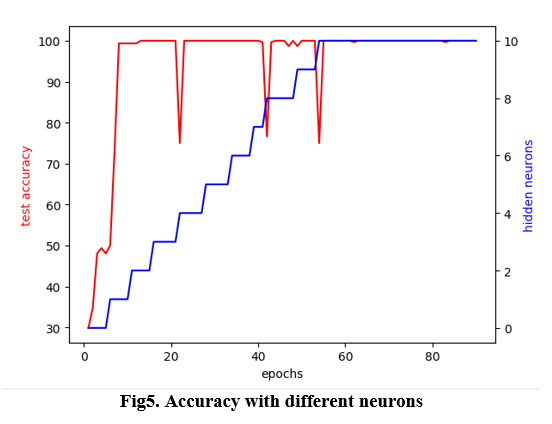
\includegraphics[width=\textwidth]{images/img9.png}
\end{align*}

\begin{align*}
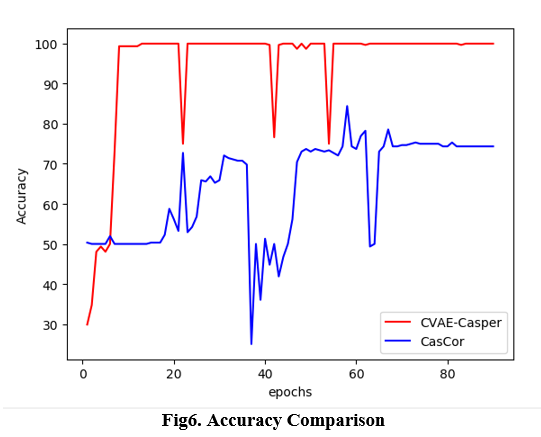
\includegraphics[width=\textwidth /2]{images/img10.png}  
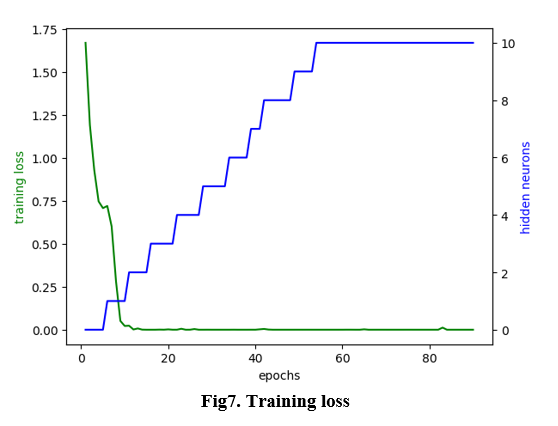
\includegraphics[width=\textwidth /2]{images/img11.png}
\end{align*}

From Fig5 It’s observed that test accuracy of CVAE-Casper rises from 30\% up to 95\% in the first 10 epochs with 2 neurons added. Afterwards, the model quickly finds the global minimum of the loss function in around 15 epochs, where the test accuracy reaches nearly 100\%. Since adding two neurons is enough to get an appropriate 95\% test accuracy, CVAE-Casper is quite strong to solve this problem. If an appropriate termination condition like test accuracy threshold is set for this model to perform early stopping, CVAE-Casper should stop with 2 neurons to achieve a relatively high accuracy. This demonstrates that CVAE-Casper can make use of conditioning to generate high quality data with label to help disease prediction. After the model converges to high test accuracy, we find some performance drops while adding new cascade neurons in epoch 4, 8 and 10, and it quickly adapts and resumes high accuracy since Cascade Correlation networks sometimes face accuracy drop due to newly added neurons are initialized randomly to a bad situation. Fig6 contains the accuracy comparison between CasCor and CVAE-Casper. There are several reasons for the dominant performance of CVAE-Casper compared to CasCor. First of all, vanilla Casper does not freeze any previous added neuron, and CasCor may freeze poor feature extractors which is difficult for output weight to adjust their poor features. Since the algorithm still allows the previous poor hidden neurons to update their input weights by a small learning rate (L3), the poor neurons still have chance to update themselves. Secondly, the original dataset is small and CVAE-Casper is able to generate more data from conditioning to help the classification task. Thirdly, according to Gedeon, T. D. (1997)~\cite{CASPER1997}, Casper can resume the property of CasCor that the latest neurons are the latest feature extractors since the learning rate of the previous hidden neurons is small with respect to the learning rate (L1) of the latest hidden neurons.






\subsection{Cardiovascular Disease Dataset}
The second dataset we use for CVAE-Casper is a Cardiovascular disease dataset from Kaggle open dataset\footnote{Retrieved from Kaggle: https://www.kaggle.com/sulianova/cardiovascular-disease-dataset}, which is a much larger dataset with physiological data. Each datapoint contains several medical indicator including: height, weight, Systolic blood pressure, Diastolic blood pressure, cholesterol, gluc, BMI, age and smoke to predict whether the patient has potential Cardiovascular Disease. The size of the dataset is 70,000 and the classes are well balanced between Cardiovascular Disease case and normal people. We are using this dataset to verify that CVAE-Casper has stable performance among various medical datasets.


\begin{table}[]
\begin{tabular}{|l|l|l|l|l|l|l|l|l|l|l|l|}
\hline
age & gender & height & weight & Systolic BP & Diastolic BP & cholesterol & gluc & smoke & alco & active & cardio(Label) \\ \hline
18393 & 2 & 168 & 62.0 & 110 & 80  & 1 & 1 & 0 & 0 & 1 & 0 \\ \hline
20228 & 1 & 156 & 85.0 & 140 & 90  & 3 & 1 & 0 & 0 & 1 & 1 \\ \hline
18857 & 1 & 165 & 64.0 & 130 & 70  & 3 & 1 & 0 & 0 & 0 & 1 \\ \hline
17623 & 2 & 169 & 82.0 & 150 & 100 & 1 & 1 & 0 & 0 & 1 & 1 \\ \hline
\end{tabular}
\caption{A quick peek of Cardiovascular Dataset}
\end{table}



The second dataset is aimed to find that conditional VAE is beneficial to consistent performance. The task here is to predict whether the given patient has Cardiovascular disease, which is a binary classification problem. The optimizer,encoding and the epochs are the same as the first experiment. Since it's a classification problem, cross-entropy loss is still used here.  The generative data is 100,000, which is much larger than the original training data(70,000). The baseline we choose is the vanilla Casper~\cite{CASPER1997} since we will analyze whether the CVAE generated data can avoid or improve the performance drop in Casper.

\begin{center}
\begin{tabular}{ c c c }
\hline
 Algorithm & Final Training Loss & Final Test Accuracy \\ 
\hline
 Casper & 0.75635 & 64.56\% \\  
\hline
 CVAE-Casper & 0.63835 & 68.69\% \\
\hline
\end{tabular}
\end{center}
From the chart above, the final test accuracy is around 5\% higher than the vanilla Casper. CVAE-Casper and vanilla Casper both uses 10 neurons to achieve such results. As a result, the CVAE-Casper has an edge over vanilla Casper due to its conditioning generative data. As detailed figures are as below.

\begin{align*}
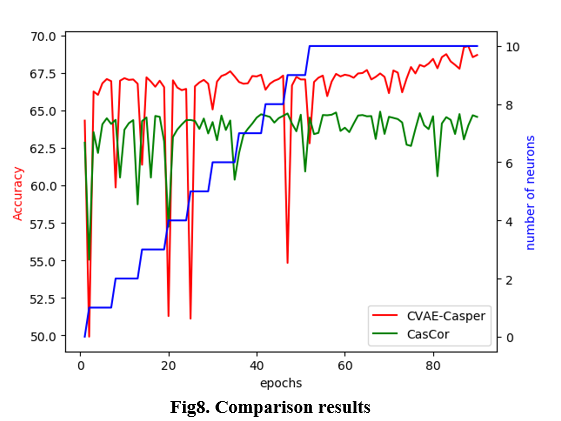
\includegraphics[width=\textwidth]{images/img12.png}
\end{align*}
From Fig8 it's observed that CVAE-Casper has better test accuracy during all training epochs except for several epochs that new random neuron is added into the architecture. Since the training set after adding generative data is much larger than the original dataset, it's expected that the random neuron is affected more by the large generative training set and the loss will be higher.